\documentclass[a4paper,12pt]{article}
\usepackage{amsmath} \usepackage{amsthm}
\usepackage[croatian]{babel}
\usepackage{graphicx}
\usepackage{amssymb} \usepackage{fancybox}
\usepackage{latexsym}
\usepackage{enumerate}
\usepackage{subcaption}
\addtolength{\hoffset}{-1cm} \addtolength{\textwidth}{2cm}
\addtolength{\topmargin}{-2.5cm} \addtolength{\textheight}{3cm}

\newtheoremstyle{zad}% name
  {0.3cm}%      Space above
  {10pt}%      Space below
  {}%         Body font
  {}%         Indent amount (empty = no indent, \parindent = para indent)
  {\bf}% Thm head font
  {.}%        Punctuation after thm head
  {\newline}%     Space after thm head: " " = normal interword space;
        %       \newline = linebreak
  {}%         Thm head spec (can be left empty, meaning `normal')

\theoremstyle{zad}
\newtheorem{zadatak}{Zadatak}

\begin{document}
%\thispagestyle{empty}
\begin{center}
\shadowbox{\Large Lijepljenje torusa}\\[2pt]
\end{center}
Torus je ploha koja ima implicitnu jednad\v{z}bu
$$\big(x^2+y^2+z^2+R^2-r^2\big)^2-4R^2\big(x^2+y^2\big)=0.$$
Za razli\v{c}ite odabire konstanti $R$ i $r$ dobivamo druk\v{c}ije toruse.\\[5pt]
Dvostruki torus nastaje lijepljenjem dva torusa. Proces lijepljenja odgovara produktu
implicitnih jednad\v{z}bi torusa umanjenom za neku konstantu. Konkretnije, implicitna
jednad\v{z}ba dvostrukog torusa glasi
$$f_1(x,y,z)\cdot f_2(x,y,z)=c,$$
pri \v{c}emu je
\begin{align*}
f_1(x,y,z)&=\big((x+a)^2+y^2+z^2+R^2-r^2\big)^2-4R^2\big((x+a)^2+y^2\big)\\
f_2(x,y,z)&=\big((x+b)^2+y^2+z^2+R^2-r^2\big)^2-4R^2\big((x+b)^2+y^2\big)
\end{align*}
za neke odabrane konstante $a,b,c,r,R$.\\[5pt]
Trostruki torus nastaje lijepljenjem tri torusa. Mo\v{z}emo ga vizualizirati preko
implicitne jednad\v{z}be
$$g_1(x,y,z)\cdot g_2(x,y,z)\cdot g_3(x,y,z)=c,$$
pri \v{c}emu je
\begin{align*}
g_1(x,y,z)&=\big((x+a)^2+y^2+z^2+R^2-r^2\big)^2-4R^2\big((x+a)^2+y^2\big)\\
g_2(x,y,z)&=\big((x+b_1)^2+(y+b_2)^2+z^2+R^2-r^2\big)^2-4R^2\big((x+b_1)^2+(y+b_2)^2\big)\\
g_3(x,y,z)&=\big((x+c_1)^2+(y+c_2)^2+z^2+R^2-r^2\big)^2-4R^2\big((x+c_1)^2+(y+c_2)^2\big)
\end{align*}
i vrijedi $b_1=a\cos{\frac{2}{3}\pi}$, $b_2=a\sin{\frac{2}{3}\pi}$, $c_1=a\cos{\frac{4}{3}\pi}$,
$c_2=a\sin{\frac{4}{3}\pi}$ za neke odabrane\vspace*{2pt} konstante $a,c,r,R$. Ako promijenimo konstante $b_2$ i $c_2$ tako da stavimo $b_2=0$ i $c_2=0$, dobivamo modificirani trostruki torus.
\begin{figure}[!h]
\centering
\subcaptionbox{dvostruki torus}{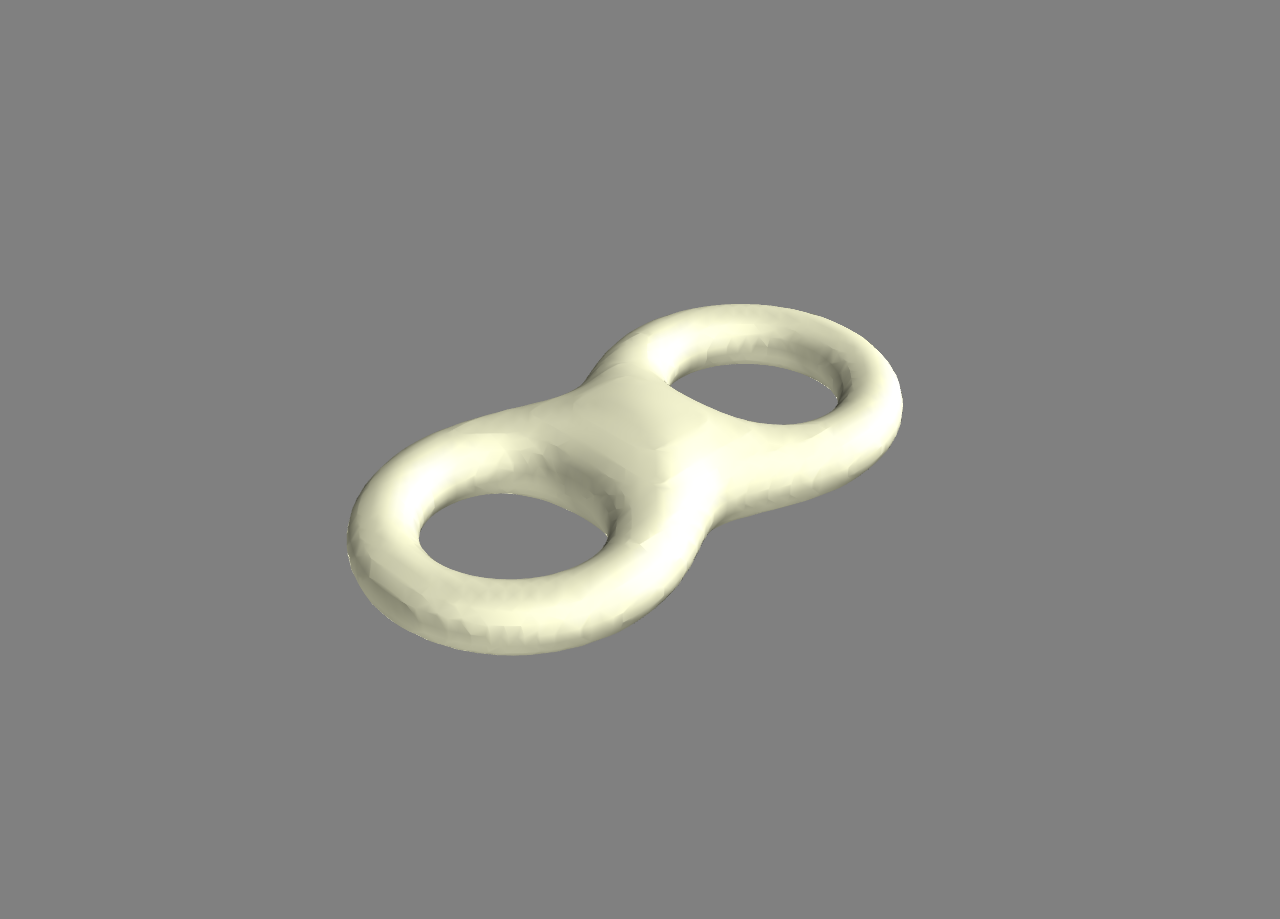
\includegraphics[scale=0.1]{dvostrukiTorus.png}}\hspace*{0.5cm}
\subcaptionbox{trostruki torus}{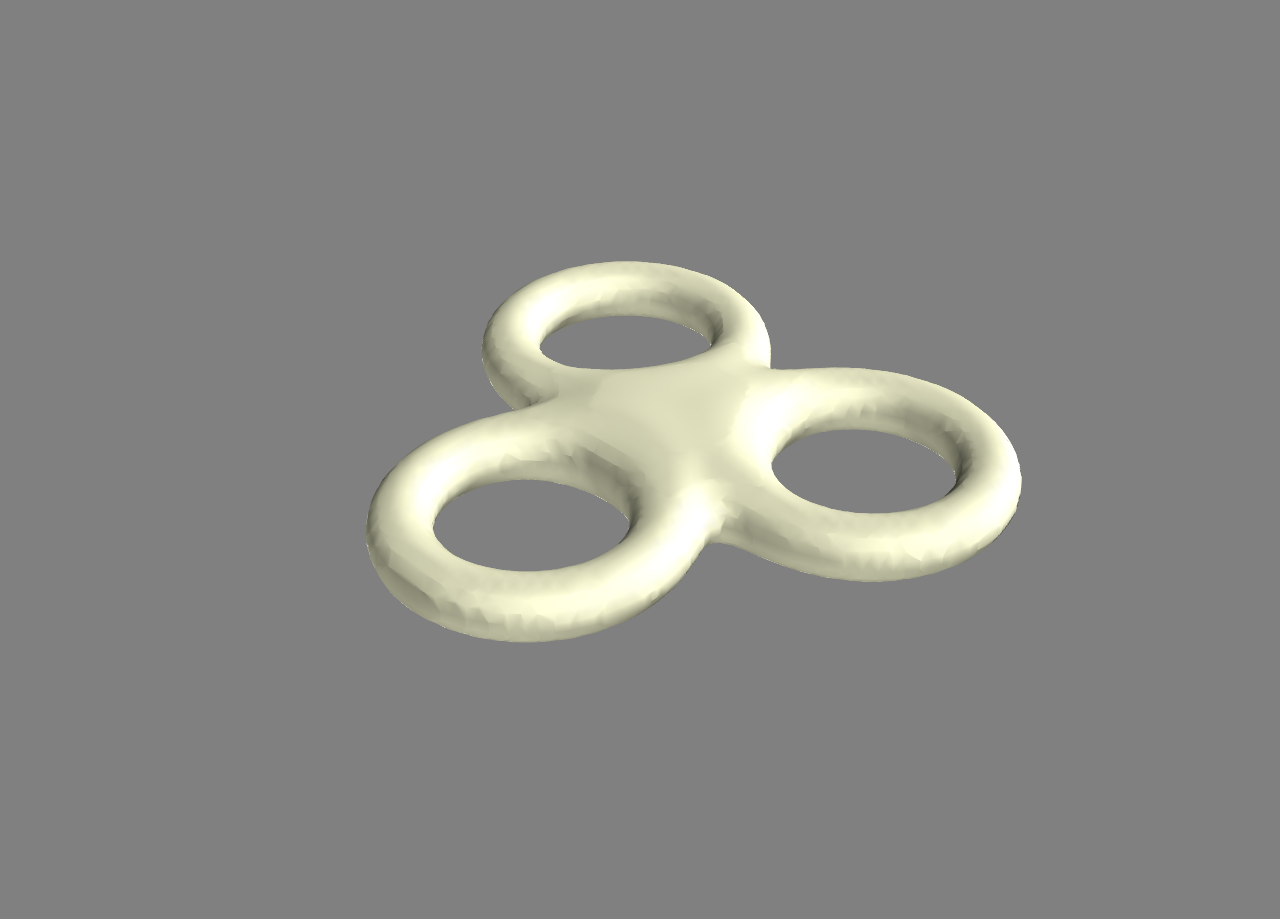
\includegraphics[scale=0.1]{trostrukiTorus.png}}\hspace*{0.5cm}
\subcaptionbox{modificirani trostruki torus}{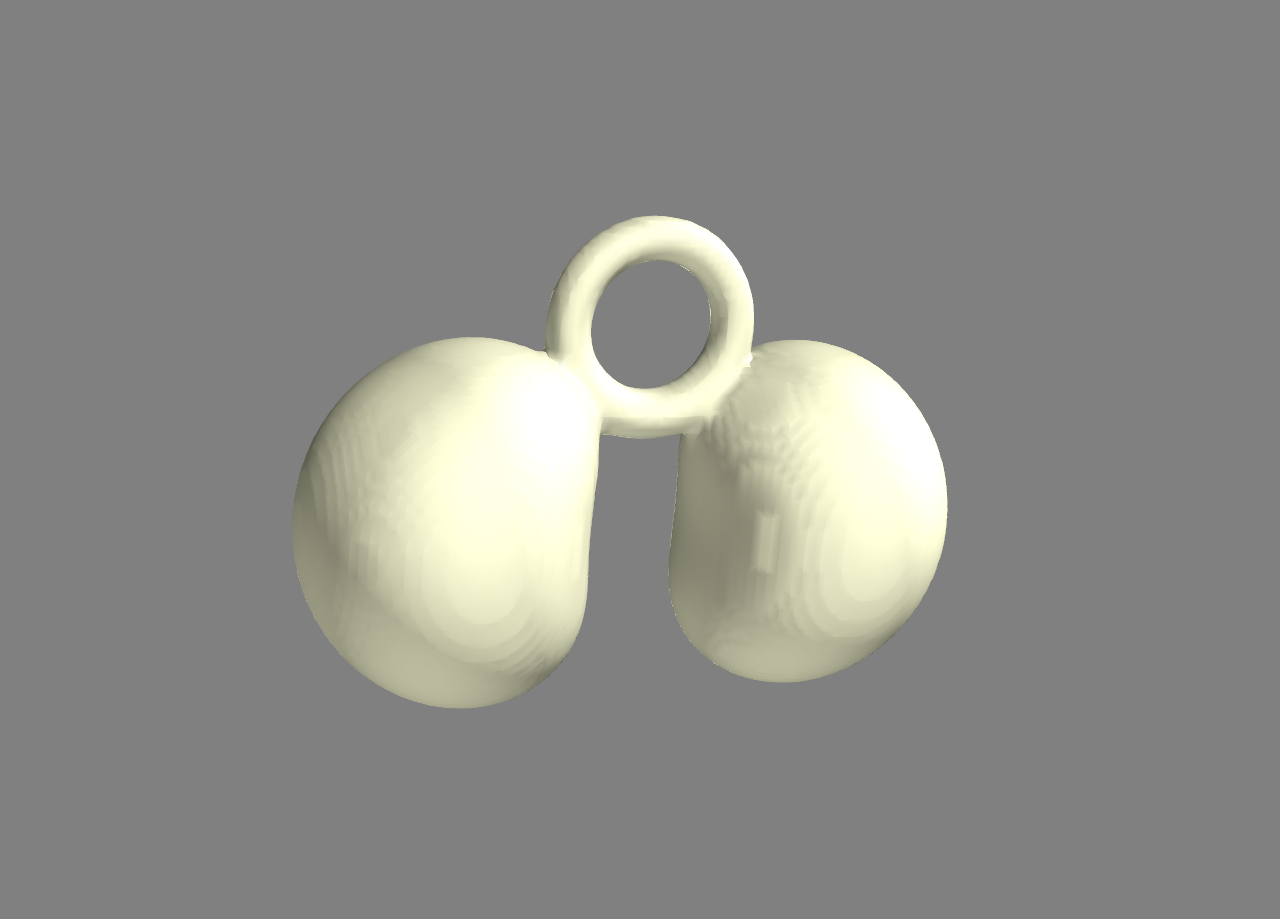
\includegraphics[scale=0.1]{smijesniModel.png}}
%\caption{Dvostruki i trostruki torus}
\end{figure}
 
\end{document}
